
\documentclass{article}
\usepackage{amsmath} %This allows me to use the align functionality.
                     %If you find yourself trying to replicate
                     %something you found online, ensure you're
                     %loading the necessary packages!
\usepackage{amsfonts}%Math font
\usepackage{graphicx}%For including graphics
\usepackage{hyperref}%For Hyperlinks
\usepackage{listings}
\usepackage{graphicx}
\usepackage{natbib}        %For the bibliography
\bibliographystyle{apalike}%For the bibliography
\usepackage[margin=1.0in]{geometry}
\usepackage{float}
\usepackage{pgf,tikz,pgfplots}
\pgfplotsset{compat=1.15}
\usepackage{mathrsfs}
\usetikzlibrary{arrows}
\pagestyle{empty}
\definecolor{rvwvcq}{rgb}{0.08235294117647059,0.396078431372549,0.7529411764705882}
\begin{document}
%set the size of the graphs to fit nicely on a 8.5x11 sheet
\noindent \textbf{Caio Brighenti }\\
\noindent \textbf{COSC 302 - Analysis of Algorithms -- Spring 2019}\\%\\ gives you a new line
\noindent \textbf{Assignment 2}\vspace{1em}\\
\begin{enumerate}
	\item Write a $\Theta (n\log n)$ algorithm for the closest pair problem using divide and conquer
	\begin{itemize}
	    \item \textbf{Algorithm:}
	        \begin{enumerate}
	            \item Divide all points $p$ into $p_l$ and $p_r$, where $p_l$ is all points to the left of the median value of $x$ in $p$, and $p_r$ is all points to the right.
	            \item Recursively find the shortest distances in the left and right splits, $d_l$ and $d_r$ respectively.
	            \item Find $d$, the minimum of $d_l$ and $d_r$.
	            \item Find $d_c$, the shortest distance of pairs crossing the midpoint used to divide $p$ into $p_l$ and $p_r$. (This step needs more detail, so we elaborate)
	                \begin{enumerate}
	                    \item Let $s$ be the set of all points within $d$ of the midpoint on the $x$ axis.
	                    \item Sort $s$ by each point's $y$ value.
	                    \item For each point in $s$, compare that point with its next 6 neighbors, keeping track of the minimum distance $d_c$. (This can be done due to knowledge of the sparsity of the points in $p_l$ and $p_r$, which will be shown in the proof.
	                \end{enumerate}
	           \item Find and return the overall minimum between $d$ and $d_c$.
	        \end{enumerate}
	        The base case of this algorithm occurs when $p$ includes only two or three points, in which case the minimum distance is manually calculated in constant time.
	   \item \textbf{Proof:}
	   \\ We will prove by induction on the size of $p$, where $p$ is the plane of points passed to the algorithm.
	   \\ \textbf{Base case #1:} size of $p$ is 2.
	   \\ This base case is trivial-there are only two points, thus there is only a single distance between points which \emph{must} be the minimum. This base case holds.
	   \\ \textbf{Base case #2:} size of $p$ is 3.
	   \\ In this case, the algorithm computes each of the possible distances manually. With three points, we have a triangle and therefore three possible distances between the points. The algorithm thus calculates each one, and returns the minimum. This base case also holds. 
	   \\ \textbf{Inductive Hypothesis:} We assume by the inductive hypothesis that the recursive algorithm correctly returns the minimum distances $d_l$ and $d_r$ in each of the left and right partitions of $p$. It thus remains to be shown that the algorithm uses this information to correctly calculate the overall minimum distance.
	   \\ \textbf{Inductive Proof}
	   \\ Let $m$ be the median point with respect to $x$ in $p$. Thus, it must be true that the minimum distance between two points in $p$ is either entirely to the left of $m$, to the right of $m$, or crosses a vertical line on $m$. There are no other ways in which this line could exist. Thus, it will suffice to find the shortest distance in $p_l$, $p_r$, and crossing the midpoint. 
	   \\ Through the inductive hypothesis, we know $d_l$ and $d_r$ to be the correct shortest distances in $p_l$ and $p_r$. It remains to find the shortest distance crossing the midpoint.
	   \\ Let $d$ be the minimum between $d_l$ and $d_r$. Thus, any minimum distance crossing the midpoint must include two points \emph{at most} $d$ from the midpoint. No point further than $d$ can cross the midpoint in shorter distance than $d$. Thus, let $s$ be the set of all points within $d$ of the midpoint.
	   \\ It is possible that all points in $p$ are in $s$, therefore it does us no good to partition this problem as such if we are not able to find an efficient way to find the shortest distance in $s$. Luckily, we have information on the sparsity in $p_l$ and $p_r$. Given that $d$ is the minimum distance in the two sides, then no pair of points can be closer than $d$ from each other. We can thus visualize this scenario as follows: \\

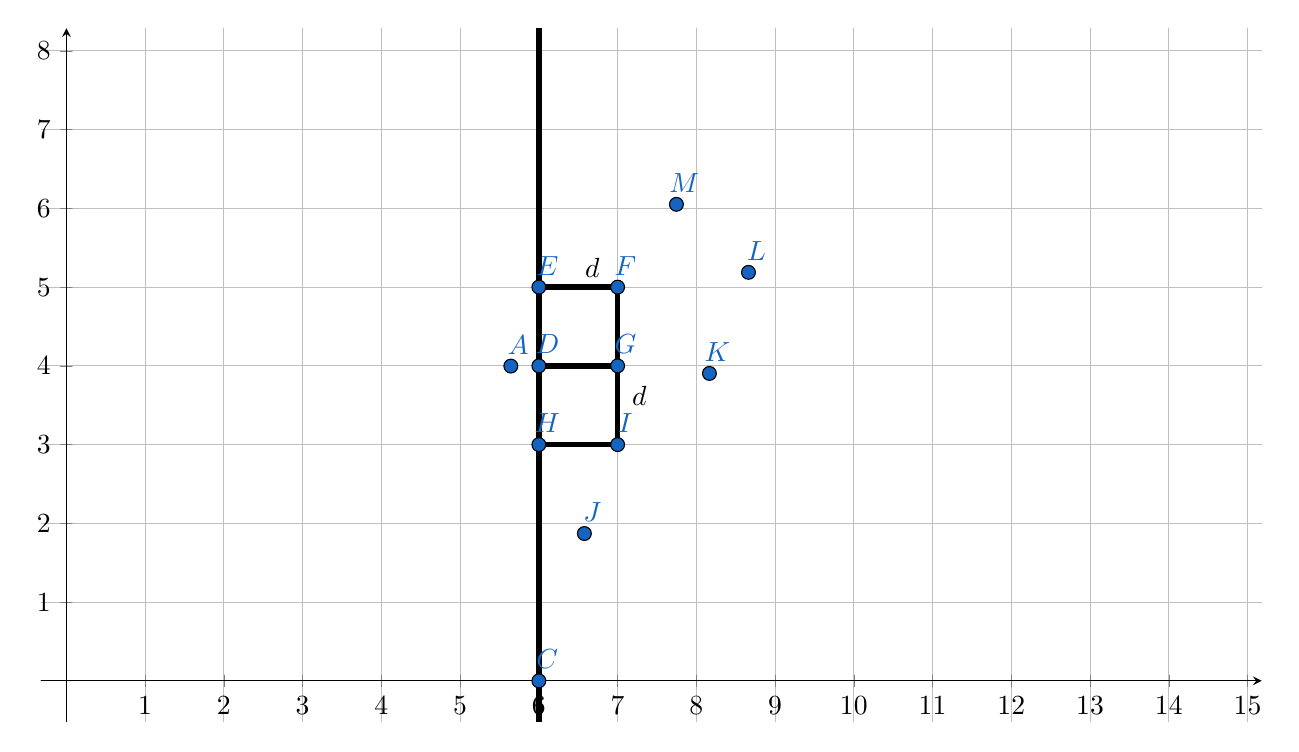
\begin{tikzpicture}[line cap=round,line join=round,>=triangle 45,x=1cm,y=1cm]
\begin{axis}[
x=1cm,y=1cm,
axis lines=middle,
ymajorgrids=true,
xmajorgrids=true,
xmin=-0.3219966230544019,
xmax=15.180820410348138,
ymin=-0.5181050824143068,
ymax=8.288003281641393,
xtick={0,1,...,15},
ytick={0,1,...,8},]
\clip(-0.3219966230544019,-0.5181050824143068) rectangle (15.180820410348138,8.288003281641393);
\draw [line width=2pt] (6,-0.5181050824143068) -- (6,8.288003281641393);
\draw [line width=2pt] (6,4)-- (6,5);
\draw [line width=2pt] (7,5)-- (7,4);
\draw [line width=2pt] (7,4)-- (6,4);
\draw [line width=2pt] (6,4)-- (6,3);
\draw [line width=2pt] (6,3)-- (7,3);
\draw [line width=2pt] (7,3)-- (7,4);
\draw (6.463662635828349,5.492413324798314) node[anchor=north west] {$d$};
\draw [line width=2pt] (6,5)-- (7,5);
\draw (7.060902308426645,3.865888258998704) node[anchor=north west] {$d$};
\begin{scriptsize}
\draw [fill=rvwvcq] (5.643636363636367,3.997272727272729) circle (2.5pt);
\draw[color=rvwvcq] (5.73935069246446,4.266165911910327) node {$A$};
\draw [fill=rvwvcq] (6,9) circle (2.5pt);
\draw[color=rvwvcq] (-0.2711677147481641,8.434136393021827) node {$B$};
\draw [fill=rvwvcq] (6,0) circle (2.5pt);
\draw[color=rvwvcq] (6.107860277684685,0.27609660987065887) node {$C$};
\draw [fill=rvwvcq] (6,4) circle (2.5pt);
\draw[color=rvwvcq] (6.107860277684685,4.278873138986886) node {$D$};
\draw [fill=rvwvcq] (6,5) circle (2.5pt);
\draw[color=rvwvcq] (6.107860277684685,5.270036850958523) node {$E$};
\draw [fill=rvwvcq] (7,5) circle (2.5pt);
\draw[color=rvwvcq] (7.099023989656322,5.270036850958523) node {$F$};
\draw [fill=rvwvcq] (7,4) circle (2.5pt);
\draw[color=rvwvcq] (7.099023989656322,4.278873138986886) node {$G$};
\draw [fill=rvwvcq] (6,3) circle (2.5pt);
\draw[color=rvwvcq] (6.107860277684685,3.2750021999386894) node {$H$};
\draw [fill=rvwvcq] (7,3) circle (2.5pt);
\draw[color=rvwvcq] (7.099023989656322,3.2750021999386894) node {$I$};
\draw [fill=rvwvcq] (6.578027679517385,1.87085360797887) circle (2.5pt);
\draw[color=rvwvcq] (6.67968549612986,2.1440589901248983) node {$J$};
\draw [fill=rvwvcq] (8.166431064087318,3.9040099402283834) circle (2.5pt);
\draw[color=rvwvcq] (8.268088880699793,4.17721532237441) node {$K$};
\draw [fill=rvwvcq] (8.662012920073137,5.187439874960888) circle (2.5pt);
\draw[color=rvwvcq] (8.763670736685613,5.460645257106915) node {$L$};
\draw [fill=rvwvcq] (7.747092570560855,6.0515313161669315) circle (2.5pt);
\draw[color=rvwvcq] (7.848750387173331,6.324736698312957) node {$M$};
\end{scriptsize}
\end{axis}
\end{tikzpicture}
    \\ Let point $A$ be a point in $p_l$ and in $s$. If we project $A$ onto the midppoint line $BC$, then any point within at most $d$ of $A$ must be within that rectangle. Given the sparsity property of $p_l$ and $p_r$, we also know that this rectangle can contain at most 6 points. This is visible in the diagram, as each of the points $D,E,F,G,H,I$ are at their minimum distance from one another $d$, and there is no way to introduce another point into the rectangle without breaking the sparsity property. This means that for each point $s_i$ in $s$, it suffices to compute only its next 6 neighbors, sorted by the $y$ axis. Any neighbor past that \emph{must} be outside of the rectangle, and consequently further than $d$ from $s_i$.
    \\ Thus, the algorithm iterates through each $s_i$ in $s$ and looks for the minimum distance between the next 6 neighbors of $s_i$. It keeps track of the overall minimum in $s$, and returns it as $d_c$.
    \\ We now have $d_l$, $d_r$, and $d_c$, where these are the minimum distances in $p_l$, $p_r$, and crossing the midpoint $m$. As we have shown, the minimum distance in $p$ \emph{must} exist in one of these three states. Thus, it suffices to take the minimum across $d$ and $d_c$ to find the overall minimum. The algorithm therefore holds, if we assume that it correctly computes the recursive minimum distances in $p_l$ and $p_r$.
	\item \textbf{Running time:} 
	\\ The recurrence of this problem is fairly typical. For each call, the algorithm takes linear time based on the size of $s$ which could be up to the size of $p$. This is because the algorithm to find the minimum distance crossing the midpoint checks 6 neighbors for each point in $s$, thus resulting in a $6n$ running time. Each call also splits $p$ in two and makes a recursive call to each partition. Thus, the recurrence is as follows:
	\\ $T(n) = 2T(\frac{n}{2})+O (n)$, where $n$ is the size of $p$.
	\\ We now solve the recurrence using the recursion tree, induction, and iteration methods.
	\begin{itemize}
	    \item \textbf{Recursion tree} \\
	    \\ This is a common case for the recursive tree. Given the coefficient on the recursive term, each node has two children. Each time, $n$ gets smaller by a factor of two. We can see three levels of this tree below. \\
	    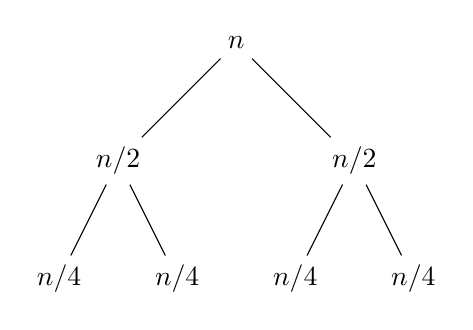
\begin{tikzpicture}[level distance=1.5cm,
        level 1/.style={sibling distance=3cm},
        level 2/.style={sibling distance=1.5cm}]
        \node {$n$}
        child {node {$n/2$}
            child {node {$n/4$}}
            child {node {$n/4$}}
        }
        child {node {$n/2$}
            child {node {$n/4$}}
            child {node {$n/4$}}
        };
        \end{tikzpicture}
        \\ The tree will continue building until $n$ reaches 1. Since it divides by 2 at leach level, the total number of levels will be $\log n$. Mathematically, we consider each node in the final level to have value 1. Therefore, we can solve for $i$ as follows, as each node has a value $\frac{n}{2^i}$ where $i$ is the corresponding level.
        \begin{align}
            \frac{n}{2^i}&=1 \\
            n&=2^i \\
            \log n = i 
        \end{align}
        \\ Thus, $i= \log n$.
        \\ Each level $i$ will have number of nodes equal to $2^i$, each of which will do work equal to $\frac{n}{2^i}$. Thus, each level will do $n$ work, as $2^i \cdot \frac{n}{2^i}=n$. Therefore, if we have $\log n$ levels, each of which does $n$ work, we have a total running time of $n \log n$.
        \item \textbf{Induction} \\
        We will now show by induction. We will guess that the correct running time is $O (n \log n)$.
        \\ \textbf{Base case:} Assume $n=2$ and $c=2$. We must show that $T(n) \leq c n \log n$.
        \\ Given the recurrence, $T(2)=2T(\frac{2}{2})+2=2+2=4$. We assume that $T(1)=1$ as the algorithm bottoms out.
        \\ As $2 * 2 \log 2 =2* 2 * 1=4$, then we have $T(n)\leq c n \log n$ for the base case. Any $c\geq 2$ here would satisfy the base case.
        \\ \textbf{Inductive hypothesis:} We assume that $T(m)\leq c m \log m$ holds for all $m$ such that $n_0\leq m<n$ and $c=2$. We now show that this implies it also holds for $n$.
        \begin{align}
            T(n) &= 2T(\frac{n}{2})+n && \text{definition} \\
            &\leq 2(c\frac{n}{2}\log \frac{n}{2})+n && \text{inductive hypothesis} \\
            &\leq cn \log \frac{n}{2}+n && \text{algebra} \\
            &\leq cn \log n - cn\log 2 + n && \text{log rules} \\
            &\leq cn \log n - cn + n && \text{$log_2 2 = 1$} \\
            &\leq cn \log n && \text{for all $c\geq 1$, $cn$ will outweigh $n$} 
        \end{align}
        Thus, we have that $T(n)\leq cn\log n$, and thus $T(n)\in O(n\log n)$.
        \item \textbf{Iteration method:}
        \\ To solve the recurrence using the iteration method, we must find find the number of calls and multiply it by the time per call. We can calculate the number of calls by leveraging our work in the recursive tree method. As each node has two children, then the number of calls must be $2^0+2^1+\cdots+2^i$, where $i$ is the final level $\log n$. Using series properties, we know this summation to be equal to $2^{\log n +1 }-1$. As $log_22^x = x, \forall x$, then the number of calls is $n+1-1=n$.
        \\ We must then multiply this by the running time per call. Naively, we would consider this to be $n$, as the running time of each recursive time is linear, resulting in $O(n^2)$. However, this ignores that the problem is smaller each time. Each node does not take $n$ time, but rather $\frac{n}{2^i}$ time where $i$ is the node's level.
        \\ We simplify this problem by considering the runtime per level, as opposed to per node, and then multiplying by the number of levels as opposed to the number of calls. Since we have $2^i$ nodes per level, each of which take $\frac{n}{2^i}$ time, then the time per level must be $n$. As we have shown, we have $\log n$ levels. Thus, the solution to the recurrence must be $T(n)\in O(n \log n)$, which we obtain by multiplying the number of levels by the running time per level.
        \end{itemize}
        \item \textbf{Applications:}
        \\ These are five applications of the closest-pair problem, as presented by Sanguthevar Rajasekaran and Sudipta Pathak from the University of Conneticut in a published paper, visible \href{https://arxiv.org/abs/1407.5609}{here}.  
        \begin{enumerate}
            \item computational biology
            \item computational finance
            \item share market analysis
            \item weather prediction
            \item entomology
        \end{enumerate}
        \item \textbf{Python Implementation:}
        \begin{verbatim}
import math

# returns distance between two points
def dist(a,b):
    return math.sqrt(math.pow(a[0]-b[0],2)+math.pow(a[1]-b[1],2))

# pre-condition: p has at most 3 points
## runs in constant time
def minBrute(p):
    num_points = len(p)
    if (num_points==2):
        return [p[0],p[1]]
    elif (num_points==3):
        d_1 = dist(p[0],p[1])
        d_2 = dist(p[0],p[2])
        d_3 = dist(p[1],p[2])
        d = min(d_1,d_2,d_3)
        if d == d_1:
            return [p[0],p[1]]
        elif d == d_2:
            return [p[0],p[2]]
        elif d == d_3:
            return [p[1],p[2]]

# returns all points in p within d of midpoint med
def midPartition(p,d,med):
    part = []
    for pair in p:
        if abs(pair[0]-p[med][0]) <= d:
            part.append(pair)
    return part

# takes a array of points p and sorts by the y values
def sortY(p):
    return sorted(p,key=lambda x: x[1])


## runs in linear time (6n)
def closestCrossPair(p):
    # sort p by y values
    p_y = sortY(p)
    # find lowest distance, init min as arbritrary pair
    d_c = dist(p[0], p[1])
    points_c = [p[0],p[1]]
    for i in range(len(p)):
        for j in range(1, min(7,len(p[i:]))):
            temp = dist(p[i],p[i+j])
            if temp < d_c:
                d_c = temp
                points_c = [p[i], p[i+j]]
    return points_c


# pre-condition: p is sorted by x
def closestPair(p):
    num_points = len(p)

    # base case
    if (num_points<=3):
        return minBrute(p);

    # split into p_l and p_r
    med = int(math.floor(num_points/2))
    p_l=p[:med]
    p_r=p[med:]

    # find d_l and d_r
    points_l = closestPair(p_l)
    d_l = dist(points_l[0], points_l[1])
    points_r = closestPair(p_r)
    d_r = dist(points_r[0], points_r[1])

    # get min d in (d_l,d_r)
    d = min(d_l,d_r)
    if d == d_l:
        points = points_l
    else :
        points = points_r

    # find min d_c crossing midpoint
    p_c = midPartition(p,d,med)
    points_c = closestCrossPair(p)
    d_c = dist(points_c[0], points_c[1])

    # find overall min
    if min(d_c,d) == d_c:
        return points_c
    else:
        return points


# creates sorted array of points
## sorted by x
p = [[1,2],[1,7],[2,9],[3,6],[4,6],[5,2],[8,3],[10,1]]
points_min = closestPair(p)
print("OVERALL MIN: ")
print(points_min )

        \end{verbatim}
	\end{itemize}
	\item Prove the grade school multiplication algorithm
	\\ Below is a pseudocode version of the algorithm:
	\begin{verbatim}
	 multiply(x,y){
	    p=0
	    while y > 0:
	        if last_digit_y == 1
	            p = p +x
	       y = floor(y/2) // bit shift
	       x = 2x // bit shift
	    return p
	 }
	\end{verbatim}
	We must show that it is correct for all binary values of $x$ and $y$. We proceed by direct proof.
	\\\\ In simple English, what this algorithm does is to multiply $x$ by each digit of $y$, each time shifting $x$ to left one digit. Finally, the sum of each of these multiplications is equal to the overall sum. We must first show this approach is correct, and then that we have a proper implementation of it.
	\\\\ It is a property of any real numbers $x,y,b$ that $(a+b)x=ax+bx$. That is to say, we can compute a multiplication of a number by separating it into parts that sum up to the whole, multiplying each of those parts, and then summing each multiplication back together. 
	\\\\ This is precisely how we represent binary numbers. For instance, the binary number $101$ is equal to $1\cdot 2^0 + 0\cdot 2^1 + 1\cdot 2^2$. More formally, any binary numbers of $n$ length can be represented as follows, where $a_i$ represents each bit value:
	\\\\ $a_0 \cdot 2^0 + a_1 \cdot 2^1 + \cdots + a_n \cdot 2^n$
	Let us then show how this applies to multiplication. Again, let $a_i$ be each bit of a binary number of length $n$, and let $y$ be an arbritary integer. Then it must be that:
	$y(a_0 \cdot 2^0 + a_1 \cdot 2^1 + \cdots + a_n \cdot 2^n) = y \cdot a_0 \cdot 2^0 + y \cdot a_1 \cdot 2^1 + \cdots + y \cdot a_n \cdot 2^n$.
	\\\\ We thus know that we can obtain a correct multiplication of $x\cdot y$ by splitting $y$ into each order of magnitude $2^i$, multiplying each by $x$ and then summing up the result. It remains to show how our algorithm performs this.
	\\\\ The crucial aspect is how the algorithm isolates each $2^i$ term, and correctly multiplies it with $x$. Our algorithm does this by each time using the last digit of $y$, followed by removing it entirely through a right-wise bit shift. This is what the floor(x/2) operation performs. Thus, upon iteration of the loop the last digit of $y$ will be the current value of $a_i$.
	\\\\ We can thus correctly obtain $a_i$, but we must still multiply it by the appropriate $2^i$ before multiplying it by $y$. This is performed in our algorithm by right shifting $x$ through the $x=2x$ operation. This simply adds a 0 to the end of $x$, or multiplies it by $2^1$. Since this is performed at each iteration of the loop, then at iteration $i$ $x$ will have been shifted $i$ times, or multiplied by $2^i$. 
	\\\\ Therefore, we correctly obtain $a_i$, and multiply $x$ by $2^i$ on each iteration. It remains to be shown that we correctly multiply by $a_i$, and finally that we sum up the total multiplication. Luckily, single digit multiplication in binary is simple: if the bit $a_i$ is 1, then $a_i \cdot x = 1$, and if the bit is 0, then $a_i \cdot x = 0$. Therefore, our algorithm simply adds $x$, which at each iteration is $x \cdot 2^i$, to the running total when $a_i$ = 1. When $a_1=0$, the algorithm does nothing, which is identical to adding $a_1 \cdot x \cdot 2^i = 0$ to the total. 
	\\\\ Thus, at each iteration we properly calculate $a_i \cdot x \cdot 2^i$, and add it to p. This means that at the end of the loop, no more work is needed. p must contain the sum of each multiplication, and thus the overall multiplication as we have shown.
	\\\\ The final point that remains to be shown is that the algorithm returns properly if the loop is not executed. The loop condition is that $y>0$. As this algorithm does not take negative numbers, if the loop does not run then it must be that $y=0$. Given we initialize p to be 0, then the algorithm will return correctly, as $x\cdot 0 = 0$ for any $x$.
	\item Prove that $\Theta (\log_a g(n)) = \Theta (\log_b g(n))$     $\forall a,b,g$ 
	\\\\ Let $f(n)= \Theta (\log_a g(n))$. We then show that $f(n)= \Theta (\log_a g(n)) \implies f(n)= \Theta (\log_b g(n))$
	\begin{align}
	    0\leq c_1 \log_a g(n) &\leq f(n) \leq c_2 \log_a g(n) && \text{definition of $\Theta$} \\
	    c_1 \frac{\log_b g(n)}{log_b a} &\leq f(n) \leq c_2 \frac{\log_b g(n)}{log_b a} && \text{change of base law} \\
	    c_1 \frac{1}{\log_b a} \log_b g(n) &\leq f(n) \leq c_2 \frac{1}{\log_b a} \log_b g(n) && \text{algebra} \\
	   0 \leq c_1 c_3 \log_b g(n) &\leq f(n) \leq c_2 c_3 \log_b g(n) && \text{$\frac{1}{\log_b a}$ must be a constant $c_3$} 
	\end{align}
	Therefore, it must be that $f(n)= \Theta (\log_b g(n))$, if $f(n)= \Theta (\log_a g(n))$. Thus, the claim is true. The practical value of this is that we have shown the base of a logarithm to be irrelevant in the asymptotic case.
	\item Prove or disprove:
	\begin{itemize}
	    \item $n^2 = O(n \log^2 n)$
	    \\ We proceed by limits.
	    \begin{align}
	        \lim_{n\to\infty} \frac{n^2}{n \log^2 n} &= \lim_{n\to\infty} \frac{n}{\log^2 n}  && \text{algebra} \\
	        &= \lim_{n\to\infty} \frac{n}{\frac{\ln^2 n}{\ln^2 2}} && \text{log rules} \\
	        &= \ln^2 2 \lim_{n\to\infty} \frac{n}{\ln^2 n} && \text{algebra} \\
	        &= \lim_{n\to\infty} \frac{n}{2\ln  n} && \text{ignore constant, log rules} \\
	        &= \lim_{n\to\infty} \frac{1}{\frac{2}{n}} && \text{L'Hopital's} \\
	        &= \lim_{n\to\infty} \frac{n}{2} = \infty && \text{algebra}
	    \end{align}
	    Therefore the claim is false, as $n^2$ grows to infinity faster than $n \log^2 n$.
	    \item $ \exists f(n) \in O(n)$ such that $ 3^n = 2^{f(n)}$.
	   \\ \\ We will show that this is possible by simplifying and then comparing $3^n$ and $2^{c_2 n}$. We use $2^{c_2 n}$ as any function $O(n)$ must be at most $c_2n$. If we take the log of each, we will have $\log3^n$ and $log2^c_2n$. Simplifying, we then have $n\log3$ and $c2n$. As $\log 3$ is a constant roughly equal to $1.59$, it is clear that we have $1.59 n \approx c_2n$ for $c_2=1.59$.
	   \\ \\ Therefore, we have that $3^n \approx 2^{1.59n}$.
	   \end{itemize}
	   \item Prove by induction that if $\exists k, n = 2^k$ then the solution of the following recurrence is $n\logn$.
	   \\ When $k=1$, $T(n)=2$, and $\forall k>1, T(n) = 2(\frac{n}{2})+n$.
	   \\ \\ We proceed by induction on $k$. First, we show the base case.
	   \\ \textbf{Base case:} $k=1$
	   \\ In this case, $T(n)$ will be equal to 2. Since $n\log n=2\log 2=2\cdot 1=2$, then the base case holds.
	   
	   \\\\ \textbf{Inductive hypothesis:} we assume that claim is true for all values of $k$ from $0$ to $k$. In other words, we assume that $T(n)=n\log n$ for all values from 0 to $k$. When then show that it is true for $k+1$.
	   \\ \emph{Notice:} $T(2^k)=2^k\log 2^k= 2^k$, as $log_22^x=x, \forall x$.
	   \\\\ We then show that the claim holds for $k+1$, where $n=2^{k+1}$.
	   \begin{align}
	       T(2^{k+1})&=2T(\frac{2^{k+1}}{2})+ 2^k+1 && \text{recurrence and definition of $n$} \\
	       &= 2T(2^k)+2^{k+1} && \text{exponent rules} \\
	       &= 2(2^kk)+2^{k+1} && \text{see notice above} \\
	       &= 2^{k+1}k+2^{k+!} && \text{exponent rules} \\
	       &= 2^{k+1}(k+1) && \text{common factor} \\
	       &= 2^{k+1}\log 2^{k+1} && \text{$\forall x, x=log_22^x$} \\
	       &= n\log n && \text{substitution}
	   \end{align}
	   Thus, the claim is true for all values of $k$, assuming the inductive hypothesis.
	   \item Solve the exercise 2.1 of 2nd book
	   \\
	   \begin{center}
	   \includegraphics[scale=0.28]{img1.jpg} \\
	   \includegraphics[scale=0.28]{img2.jpg} \\
	   \includegraphics[scale=0.28]{img3.jpg} \\ 
	   \end{center}
\end{enumerate}


\end{document}

